\begin{ex}
(Ufscar) A probabilidade de que um componente eletrônico não quebre é chamada de confiabilidade.  Para aumentar a confiabilidade de um sistema, é comum que se instalem dois componentes eletrônicos de mesma confiabilidade em paralelo. Nesse caso, o sistema só irá falhar se ambos os componentes instalados falharem simultaneamente.
  \begin{center}
      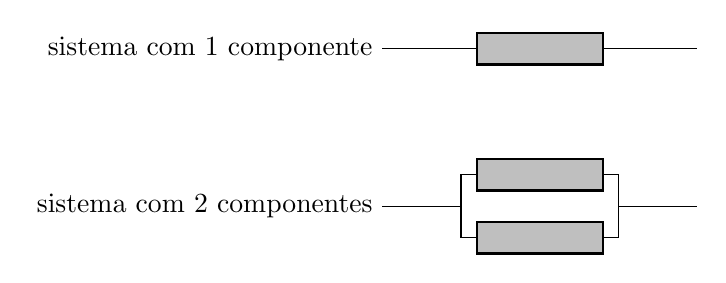
\begin{tikzpicture}
       \draw (-2,0)--(-.8,0);
       \draw [ thick, fill=lightgray] (-.8,-.2) rectangle (.8,.2); \draw (.8,0)--(2,0);
       \node at (-2,0) [left] {sistema com 1 componente};
       \draw(-2,-2)--(-1,-2); \draw (1,-2)--(2,-2);\draw [ thick, fill=lightgray] (-.8,-1.8) rectangle (.8,-1.4);\draw [ thick, fill=lightgray] (-.8,-2.6) rectangle (.8,-2.2);\draw (-.8,-1.6)--(-1,-1.6)--(-1,-2.4)--(-.8,-2.4); \draw (.8,-1.6)--(1,-1.6)--(1,-2.4)--(.8,-2.4);
        \node at (-2,-2) [left] {sistema com 2 componentes};
       
      \end{tikzpicture}
  \end{center}

   \begin{enumerate}[(a)]
   \item	Calcule a probabilidade de que um sistema com dois componentes, cada um de confiabilidade 90\%, não falhe;
   \item	Admita que um sistema com n elementos em paralelo só falhará se os n componentes falharem simultaneamente.  Calcule o número de componentes em paralelo que devem ser instalados em um sistema para que ele tenha confiabilidade de 99,9\%, sabendo-se que cada componente tem confiabilidade 50\%.                       (Adote log 2 = 0,3)
   \end{enumerate}
     \begin{sol}
      \phantom{A} 
      \begin{enumerate} [(a)]
          \item total (-) os 2 componentes falharem $\Longrightarrow 1 - \frac{1}{10}\cdot\frac{1}{10}=\frac{99}{100}=99\%$ 
          \item confiabilidade de cada componente: $50\% = \frac{1}{2}$\\  $1-(\frac{1}{2})^n = 99,9\% \hspace{0,3cm} \rightarrow (\frac{1}{2})^n=\frac{1}{1000} \hspace{0,3cm} \rightarrow 2^n={10}^3 \hspace{0,3cm} \rightarrow nlog2=3log 10\hspace{0,1cm} \rightarrow n=\frac{3}{0,3}=10 $
          
      \end{enumerate}
     \end{sol}
\end{ex}